\documentclass[11pt]{article}
\usepackage[cm]{fullpage}
%%AVC PACKAGES
\usepackage{avcgreek}
\usepackage{avcfonts}
\usepackage{avcmath}
\usepackage[numberby=section]{avcthm}
\usepackage{qcmacros}
\usepackage{goldstone}
%%MACROS FOR THIS DOCUMENT
\numberwithin{equation}{section}
\usepackage[
  margin=1.5cm,
  includefoot,
  footskip=30pt,
  headsep=0.2cm,headheight=1.3cm
]{geometry}
\usepackage{fancyhdr}
\pagestyle{fancy}
\fancyhf{}
\fancyhead[LE,RO]{Quiz 4, Handout 1: Diagrams}
\fancyfoot[CE,CO]{\thepage}
\usepackage{url}
\makeatother
\newcommand{\resolventline}[2][1]{
  \tikz[overlay]{
      \draw[thick,flexdotted] (0,-1ex) to ++(0,#1*4.5ex) node[above,inner sep=1pt] {#2};
  }
}

\begin{document}

\setlength{\abovedisplayskip}{3pt}
\setlength{\belowdisplayskip}{3pt}

\setcounter{section}{3}
\section{Diagram notation}


\begin{ntt}\label{ntt:diagram-notation}
\thmtitle{Diagram notation}
In diagram notation, particle-hole operators are written as oriented lines extending from a vertex.
Particle annihilation operators enter the vertex from below, particle creation operators leave the vertex at the top, and single-excitation operators have both creation and annihilation lines.
Contractions are represented by joining particle-hole lines with compatible position and orientation.
\begin{align}
\diagram{
  \node[dot=white] (p) at (0,0) {};
  \draw[-<-] (p) to ++(0,-0.5);
}
\equiv
  a_p
&&
\diagram{
  \node[dot=white] (p) at (0,0) {};
  \draw[->-] (p) to ++(0,+0.5);
}
\equiv
  a_p^\dagger
&&
\diagram{
  \node[dot=white] (a) at (0,0) {};
  \draw[->-] (a) to ++(0,+0.5);
  \draw[-<-] (a) to ++(0,-0.5);
}
\equiv
  a_p\dg a_q
=
  a^p_q
&&
\diagram{
  \node[dot=white] (p) at (0,+0.5) {};
  \node[dot=white] (q) at (0,-0.5) {};
  \draw[->-] (q) to (p);
}
\equiv
  \ctr{}{a}{_p}{a} a_p a_q\dg
=
  a^{q^\ptcl}_{p^\ptcl}
\end{align}
Quasiparticle operators are distinguished by the use of closed-circle vertices, with particle lines pointing upward and with hole lines pointing downward.
Single-excitation operators split into four cases representing the virtual and occupied blocks of $a^p_q$.
Internal contractions of single excitations (\textit{bubble contractions}) are implicitly taken to be hole contractions.
\begin{align}
\diagram{
  \node[dot] (a) at (0,0) {};
  \draw[-<-] (a) to ++(0,-0.5);
}
\equiv
  b_a
&&
\diagram{
  \node[dot] (a) at (0,0) {};
  \draw[->-] (a) to ++(0,+0.5);
}
\equiv
  b_a^\dagger
&&
\diagram{
  \node[dot] (i) at (0,0) {};
  \draw[->-] (i) to ++(0,-0.5);
}
\equiv
  b_i
&&
\diagram{
  \node[dot] (i) at (0,0) {};
  \draw[-<-] (i) to ++(0,+0.5);
}
\equiv
  b_i^\dagger
&&
\diagram{
  \node[dot] (a) at (0,+0.5) {};
  \node[dot] (b) at (0,-0.5) {};
  \draw[->-] (b) to (a);
}
\equiv
  \ctr{}{b}{_a}{b}  b_ab_b\dg
=
  a^{b^\ptcl}_{a^\ptcl}
&&
\diagram{
  \node[dot] (i) at (0,+0.5) {};
  \node[dot] (j) at (0,-0.5) {};
  \draw[-<-] (j) to (i);
}
\equiv
  \ctr{}{b}{_i}{b}  b_ib_j\dg
=
  a^{i^\hole}_{j^\hole}
\end{align}
\begin{align}
\diagram{
  \node[dot] (ab) at (0,0) {};
  \draw[->-] (ab) to ++(0,+0.5);
  \draw[-<-] (ab) to ++(0,-0.5);
}
\equiv
  b_a\dg b_b
=
  a^a_b
&&
\diagram{
  \node[dot] (ai) at (0,0) {};
  \draw[->-] (ai) to ++(-0.25,+0.5);
  \draw[-<-] (ai) to ++(+0.25,+0.5);
}
\equiv
  b_a\dg b_i\dg
=
  a^a_i
&&
\diagram{
  \node[dot] (ia) at (0,0) {};
  \draw[->-] (ia) to ++(-0.25,-0.5);
  \draw[-<-] (ia) to ++(+0.25,-0.5);
}
\equiv
  b_ib_a
=
  a^i_a
&&
\diagram{
  \node[dot] (ij) at (0,0) {};
  \draw[-<-] (ij) to ++(0,+0.5);
  \draw[->-] (ij) to ++(0,-0.5);
}
\equiv
  b_ib_j\dg 
=
  a^i_j
&&
\diagram{
  \node[dot] (pq) at (0,0) {};
  \draw[->-] (pq) arc (0:360:+0.3) {};
}
\equiv
  \ctr{}{b}{_i}{b}  b_ib_i\dg
=
  a^{i^\hole}_{i^\hole}
\end{align}
Higher excitation operators are depicted by joining single-excitation operators with a solid line.
Contracted operators are implicitly normal ordered together.
Normal-ordered products of uncontracted operators are joined with a dotted line.
\begin{align*}
\diagram{
  \node[dot=white] (a1) at (1,0) {};
  \node (dots) at (1.6,0) {$\cdots$};
  \node[dot=white] (an) at (2.2,0) {};
  \draw (a1)--(dots)--(an);
  \draw[->-] (a1) to ++(0,+0.5);
  \draw[->-] (an) to ++(0,+0.5);
  \draw[-<-] (a1) to ++(0,-0.5) coordinate[below left=0.1cm and 0.1cm] (startbrace);
  \draw[-<-] (an) to ++(0,-0.5) coordinate[below right=0.1cm and 0.1cm] (endbrace);
  \draw[decorate,decoration={brace,mirror}] (startbrace) to node[midway,below=0.1cm] () {\scriptsize{$m$ times}} (endbrace);
}
\equiv
  \no{a^{p_1}_{q_1}\cd a^{p_m}_{q_m}}
=
  a^{p_1\cd p_m}_{q_1\cd q_m}
&&
\diagram{
% first excitation operator
  \node[dot=white] (a1) at (1,0.5) {};
  \node (dots) at (1.6,0.5) {$\cdots$};
  \node[dot=white] (an) at (2.2,0.5) {};
  \draw (a1)--(dots)--(an);
  \draw[->-] (a1) to ++(0,+0.5) coordinate[above left=0.1cm and 0.1cm] (startbrace);
  \draw[->-] (an) to ++(0,+0.5) coordinate[above right=0.1cm and 0.1cm] (endbrace);
  \draw[-<-] (a1) to ++(0,-0.5);
  \draw[decorate,decoration={brace}] (startbrace) to node[midway,above=0.1cm] () {\scriptsize{$m$ times}} (endbrace);
% second excitation operator
  \node[dot=white] (b1) at (2.2,-0.5) {};
  \node (dots2) at (2.8,-0.5) {$\cdots$};
  \node[dot=white] (bn) at (3.4,-0.5) {};
  \draw (b1)--(dots2)--(bn);
  \draw[->-] (bn) to ++(0,+0.5);
  \draw[-<-] (b1) to ++(0,-0.5) coordinate[below left=0.1cm and 0.1cm] (startbrace2);
  \draw[-<-] (bn) to ++(0,-0.5) coordinate[below right=0.1cm and 0.1cm] (endbrace2);
  \draw[decorate,decoration={brace,mirror}] (startbrace2) to node[midway,below=0.1cm] () {\scriptsize{$n$ times}} (endbrace2);
% connecting line
  \draw[->-] (b1)--(an);
}
\equiv
  \no{a^{p_1\cd p_m}_{q_1\cd q_m^\ptcl}a^{r_1^\ptcl\cd r_n}_{s_1\cd s_n}}
&&
\diagram{
% first excitation operator
  \node[dot=white] (a1) at (1,0) {};
  \node (dots) at (1.6,0) {$\cdots$};
  \node[dot=white] (an) at (2.2,0) {};
  \draw (a1)--(dots)--(an);
  \draw[->-] (a1) to ++(0,+0.5);
  \draw[->-] (an) to ++(0,+0.5);
  \draw[-<-] (a1) to ++(0,-0.5) coordinate[below left=0.1cm and 0.1cm] (startbrace);
  \draw[-<-] (an) to ++(0,-0.5) coordinate[below right=0.1cm and 0.1cm] (endbrace);
  \draw[decorate,decoration={brace,mirror}] (startbrace) to node[midway,below=0.1cm] () {\scriptsize{$m$ times}} (endbrace);
% second excitation operator
  \node[dot=white] (b1) at (3,0) {};
  \node (dots2) at (3.6,0) {$\cdots$};
  \node[dot=white] (bn) at (4.2,0) {};
  \draw (b1)--(dots2)--(bn);
  \draw[->-] (b1) to ++(0,+0.5);
  \draw[->-] (bn) to ++(0,+0.5);
  \draw[-<-] (b1) to ++(0,-0.5) coordinate[below left=0.1cm and 0.1cm] (startbrace2);
  \draw[-<-] (bn) to ++(0,-0.5) coordinate[below right=0.1cm and 0.1cm] (endbrace2);
  \draw[decorate,decoration={brace,mirror}] (startbrace2) to node[midway,below=0.1cm] () {\scriptsize{$n$ times}} (endbrace2);
% connecting line
  \draw[densely dotted] (an)--(b1);
}
\equiv
  \no{a^{p_1\cd p_m}_{q_1\cd q_m}a^{r_1\cd r_n}_{s_1\cd s_n}}
\end{align*}
$\F$-normal-ordering is indicated by the use of double-circle vertices, $\diagram{\node[ddot=white] {};}$ and $\diagram{\node[ddot] {};}$ instead of $\diagram{\node[dot=white] {};}$ and $\diagram{\node[dot] {};}$.
These building blocks can be used to construct more complicated products.
Products of diagrams are written from top to bottom, representing left-to-right ordering in the corresponding algebraic expression.
\end{ntt}


\begin{dfn}\label{dfn:operators-in-diagram-notation}
\thmtitle{$m$-electron operators in diagram notation}
The building blocks of a graph are $m$-electron operators, which can be represented in two equivalent ways.
The \textit{Goldstone representation} depicts an operator as a label attached to the corresponding excitation operator, whereas the \textit{Hugenholtz representation} depicts the operator as a single vertex with $m$ outgoing and incoming lines.
Note that $\pr{\tfr{1}{m!}}^2\sum_{\mr{Einstein}}$ is baked into the definition (see \cref{dfn:graph} and \cref{ax:rules-of-interpretation}).
\begin{align}
\diagram{
  \node[draw] (label) at (-0.7,0) {\bm{v}};
  \node[dot=white] (v1) at (0,0) {};
  \node (dots) at (0.6,0) {$\cdots$};
  \node[dot=white] (vn) at (1.2,0) {};
  \draw (label)--(v1)--(dots)--(vn);
  \draw[->-] (v1) to ++(0,+0.45);
  \draw[->-] (vn) to ++(0,+0.45);
  \draw[-<-] (v1) to ++(0,-0.45);
  \draw[-<-] (vn) to ++(0,-0.45);
}
\equiv&\
  \pr{\tfr{1}{m!}}^2
  \sum_{\mr{Einstein}}
  \ol{v}_{p_1\cdots p_m}^{q_1\cdots q_m}
  a^{p_1\cdots p_m}_{q_1\cdots q_m}
\equiv
\diagram{
  \node[draw,circle] (label) at (0,0) {\bm{v}};
  \draw[->-] (label.140) -- ++(140:0.5) ++(140:0.2);
  \draw[->-] (label.120) -- ++(120:0.5) ++(120:0.2);
  \node at (70:0.55) {$\cdot$};
  \node at (80:0.55) {$\cdot$};
  \node at (90:0.55) {$\cdot$};
  \draw[->-] (label.40)  -- ++(40:0.5)  ++(40:0.25);
  \draw[-<-] (label.220) -- ++(220:0.5) ++(220:0.2);
  \draw[-<-] (label.240) -- ++(240:0.5) ++(240:0.2);
  \node at (270:0.55) {$\cdot$};
  \node at (280:0.55) {$\cdot$};
  \node at (290:0.55) {$\cdot$};
  \draw[-<-] (label.320) -- ++(320:0.5) ++(320:0.25);
}
&&&
\diagram{
  \node[draw] (label) at (-0.7,0) {\bm{v}};
  \node[dot=white] (v1) at (0,0) {};
  \node (dots) at (0.6,0) {$\cdots$};
  \node[dot=white] (vn) at (1.2,0) {};
  \draw (label)--(v1)--(dots)--(vn);
  \draw[->-] (v1) to ++(0,+0.45) node[above] {$p_1$};
  \draw[->-] (vn) to ++(0,+0.45) node[above] {$p_m$};
  \draw[-<-] (v1) to ++(0,-0.45) node[below] {$q_1$};
  \draw[-<-] (vn) to ++(0,-0.45) node[below] {$q_m$};
}
=&\
  \ol{v}_{p_1\cd p_m}^{q_1\cd q_m}a^{p_1\cd p_m}_{q_1\cd q_m}
\\
\diagram{
  \node[draw] (label) at (-0.7,0) {\bm{v}};
  \node[ddot=white] (v1) at (0,0) {};
  \node (dots) at (0.6,0) {$\cdots$};
  \node[ddot=white] (vn) at (1.2,0) {};
  \draw (label)--(v1)--(dots)--(vn);
  \draw[->-] (v1) to ++(0,+0.45);
  \draw[->-] (vn) to ++(0,+0.45);
  \draw[-<-] (v1) to ++(0,-0.45);
  \draw[-<-] (vn) to ++(0,-0.45);
}
\equiv&\
  \pr{\tfr{1}{m!}}^2
  \sum_{\mr{Einstein}}
  \ol{v}_{p_1\cdots p_m}^{q_1\cdots q_m}
  \tl{a}^{p_1\cdots p_m}_{q_1\cdots q_m}
\equiv
\diagram{
  \node[draw,double,circle] (label) at (0,0) {\bm{v}};
  \draw[->-] (label.140) -- ++(140:0.5) ++(140:0.2);
  \draw[->-] (label.120) -- ++(120:0.5) ++(120:0.2);
  \node at (70:0.55) {$\cdot$};
  \node at (80:0.55) {$\cdot$};
  \node at (90:0.55) {$\cdot$};
  \draw[->-] (label.40)  -- ++(40:0.5)  ++(40:0.25);
  \draw[-<-] (label.220) -- ++(220:0.5) ++(220:0.2);
  \draw[-<-] (label.240) -- ++(240:0.5) ++(240:0.2);
  \node at (270:0.55) {$\cdot$};
  \node at (280:0.55) {$\cdot$};
  \node at (290:0.55) {$\cdot$};
  \draw[-<-] (label.320) -- ++(320:0.5) ++(320:0.25);
}
&&&
\diagram{
  \node[draw,circle] (label) at (0,0) {\bm{v}};
  \draw[->-] (label.140) -- ++(140:0.5) ++(140:0.2) node {$p_1$};
  \draw[->-] (label.120) -- ++(120:0.5) ++(120:0.2) node {$p_2$};
  \node at (70:0.55) {$\cdot$};
  \node at (80:0.55) {$\cdot$};
  \node at (90:0.55) {$\cdot$};
  \draw[->-] (label.40)  -- ++(40:0.5)  ++(40:0.25)  node {$p_m$};
  \draw[-<-] (label.220) -- ++(220:0.5) ++(220:0.2) node {$q_1$};
  \draw[-<-] (label.240) -- ++(240:0.5) ++(240:0.2) node {$q_2$};
  \node at (270:0.55) {$\cdot$};
  \node at (280:0.55) {$\cdot$};
  \node at (290:0.55) {$\cdot$};
  \draw[-<-] (label.320) -- ++(320:0.5) ++(320:0.25) node {$q_m$};
}
=&\
  \ol{v}_{p_{\pi(1)}\cd p_{\pi(m)}}^{q_{\si(1)}\cd q_{\si(m)}}
  a^{p_{\pi(1)}\cd p_{\pi(m)}}_{q_{\si(1)}\cd q_{\si(m)}}
\end{align}
The labeled diagrams on the right represent just the summand of the operator, which highlights the difference between representations.
Both summands correspond to an excitation operator weighted by its antisymmetrized interaction tensor,\footnotemark\ but whereas the Goldstone summand specifies an ordering for the indices of its corresponding algebraic term, the Hugenholtz summand does not.
Since the phases of $\ol{v}_{p_1\cd p_m}^{q_1\cd q_m}$ and $a^{p_1\cd p_m}_{q_1\cd q_m}$ cancel under index permutation, the two labeled diagrams are actually equal -- a Hugenholtz summand can be expanded into a Goldstone summand by simply choosing an arbitrary ordering for the indices.
In practice, the symmetry of the Hugenholtz operator simplifies the enumeration of Wick expansions whereas the Goldstone operator makes it easier to evaluate a graph's overall phase.
\end{dfn}
\footnotetext{In the original paper [J.~Goldstone, \textit{P.~Roy.~Soc.~A} \textbf{239}, (1957)], Goldstone's diagrams were actually defined in terms of non-antisymmetrized integrals.  The \textit{antisymmetrized Goldstone diagrams} used here are sometimes called \textit{Brandow diagrams}.}




\begin{dfn}\label{dfn:graph}
\thmtitle{Graph}
A \textit{graph}\footnotemark\
$G=(O,L,h,t)$ consists of a set of $m$-electron operators $O$, a set of lines $L$, and two mappings $h,t:L\rightarrow O$ that return the \textit{head} $h(l)\in O$ and \textit{tail end} $t(l)\in O$ of each line in $L$.
Two lines are considered \textit{equivalent} if they share the same head and tail.
Here, we allow for \textit{external lines} in which one of the ends is $e$, the \textit{free end}, which is formally considered a member of $O$.
Lines with no free end are termed \textit{internal}.
A graph is termed \textit{closed} if it contains no external lines, representing a scalar-valued algebraic term.
Otherwise, the graph is \textit{open} and represents an operator-valued algebraic term.
The \textit{rules of interpretation} for translating $G$ into an algebraic expression are given below.
\end{dfn}
\footnotetext{In graph theory jargon this is essentially a \textit{directed multigraph}, except that the vertical ordering of operators matters.}


\begin{dfn}
\thmtitle{Connected and linked graphs}
Two lines are \textit{adjacent} if they share a non-free end.
In a Goldstone diagram, two lines are termed \textit{Goldstone adjacent} if they end on the same single-excitation vertex of an operator.
In this context, the broader sense of the adjacency is called \textit{Hugenholtz adjacency}.
A \textit{path} is a sequence of lines $(l_1,\ld,l_n)$ such that $l_i$ is adjacent to $l_{i+1}$ and no line is repeated.
In a Goldstone diagram, one can distinguish between \textit{Goldstone} and \textit{Hugenholtz paths} depending on whether or not the lines are all Goldstone adjacent.
A \textit{Goldstone cycle} is a Goldstone path whose ends are either Goldstone adjacent or free.
A Goldstone cycle with free ends is an \textit{open cycle}.
Otherwise, it forms a \textit{loop}.
A graph is considered \textit{connected} if there is a Hugenholtz path connecting any two of its operators.
A closed, disconnected subgraph is considered \textit{unlinked} from the rest of the graph.
Note this last distinction: A \textit{disconnected} graph is still classified as \textit{linked}, as long as none of its disconnected subgraphs are closed.
\end{dfn}


\begin{dfn}\label{dfn:equivalent-subgraphs}
\thmtitle{Equivalent subgraphs}
Repeated copies of the same operator are formally distinguished as elements of a graph's operator set and are termed \textit{identical operators}.
Operators that can be interchanged without altering the graph are termed \textit{interchangeable operators}.
This occurs when they are connected to the same set of operators in the same way.
When identical operators are also interchangeable, we call them \textit{equivalent operators}.
More generally, if $G[O']$ denotes the subgraph associated with\footnote{See \url{https://en.wikipedia.org/wiki/Induced_subgraph}} some subset $O'\subset O$ of the operators in $G$,
then two disjoint subgraphs\footnote{That is, $G[O_1]$ and $G[O_2]$ with $O_1\cap O_2=\O$.} can also be classified as \textit{identical}, \textit{interchangeable}, or \textit{equivalent}.
For our purposes, these terms will be restricted to \textit{connected subgraphs}.
\end{dfn}


\begin{dfn}
\thmtitle{Summand graph}
A \textit{summand graph}\footnotemark\ $\Si(G)=(G,S,s)$ associates each line $l$ in $G$ with a symbol $s(l)\in S$ through the \textit{label mapping} $s:L\rightarrow S$.
Pictorially, this corresponds to labeling each line in $G$ with spin-orbital index, $p,q,r,s,$ etc.
$\Si(G)$ translates directly into an algebraic summand according to \Cref{dfn:operators-in-diagram-notation} and \Cref{ntt:diagram-notation}.
\end{dfn}
\footnotetext{In graph theory jargon this is an \textit{edge-labeled directed multigraph}.}



\begin{dfn}
\thmtitle{Degeneracy}
The \textit{line degeneracy} or simply \textit{degeneracy} of $G$ is the number of permutational symmetries in $\Si(G)$, a positive integer here denoted $\mr{dg}(G)$.
Formally, this can be defined as follows.
If $S=\{s_1,\ld,s_n\}$ is the label set of $\Si(G)$ and $s(l_i)=s_i$ is its label map, we can define a new summand graph $\Si_{\pi}(G)=(G, S, s_{\pi})$ with a permuted label map $s_\pi$ given by $s_{\pi}(l_i)=s_{\pi(i)}$, where $\pi$ is a permutation in $\mr{S}_n$.
Then $\mr{dg}(G)$ is the number of $\Si_{\pi}(G)$ that are equal to $\Si(G)$.
Assuming no identical operators, the degeneracy of $G$ is simply given by $\mr{dg}(G)=|L_1|!\cd|L_h|!$ where $L_1\cup\cd\cup L_h$ partitions its line set into subsets of equivalent lines and $|L_i|$ denotes the number of elements in $L_i$.
When the graph does contain identical operators, there is an additional factor of $k!$ for each set $\{G[O_1],\ld,G[O_k]\}$ of equivalent subgraphs.
\end{dfn}


\begin{ax}\label{ax:rules-of-interpretation}
\thmtitle{Rules of interpretation}
The algebraic intepretation of a graph $G$ is obtained from $\Si(G)$ as follows.
\begin{enumerate}
  \item Multiply $\Si(G)$ by $\mr{dg}(G)^{-1}$, the \textit{degeneracy factor}.
  \item Sum each index in $\Si(G)$ over its range.
\end{enumerate}
Symbolically, these rules can be stated as follows: $G=\fr{1}{\mr{dg}(G)}\sum_{\mr{Einstein}}\Si(G)$.
\end{ax}


\begin{dfn}
\thmtitle{Contraction}
Formally, a \textit{graph contraction} is a map $G\mapsto c(G)$ joining one or more compatible external lines in $G$.
For example, $c$ might replace $l_1$ and $l_2$, which have ends $(t(l_1),h(l_1))=(o_1,e)$ and $(t(l_2),h(l_2))=(e,o_2)$, with $l_{12}$, which has ends $(t(l_{12}),h(l_{12}))=(o_1,o_2)$.
Two contractions $c$ and $c'$ of $G$ are \textit{equivalent} if they are graphically indistinguishable, i.e. $c(G)=c'(G)$.
The number of equivalent ways of achieving a given contraction $c$ is called its \textit{pattern degeneracy}, which is denoted $\mr{pat}(c)$.
The complete set of unique contraction patterns for a graph is here denoted $\mr{Ctr}(G)$.
Combined with Wick's theorem, these concepts lead to the following statement
\begin{align}\label{eq:wicks-theorem-for-summand-graphs}
  \sum_{\mr{Einstein}}
  \Si(G)
=
  \sum_{\mr{Einstein}}
  \gno{\Si(G)}
+
  \sum_{c\in\mr{Ctr}(G)}
  \mr{pat}(c)\,
  \sum_{\mr{Einstein}}
  \gno{\Si(c(G))}
\end{align}
which will be used to prove a more elegant graphical formulation of Wick's theorem below.
\end{dfn}


\begin{samepage}
\begin{lem}\label{lem:pattern-degeneracy-no-identical-operators}
\thmstatement{The pattern degeneracy of a contraction $c$ is $\mr{pat}(c)=\dfr{\mr{dg}(G)}{\mr{dg}(c(G))}$.
}
\begin{addmargin}[1em]{0em}
{\renewcommand*{\thefootnote}{\fnsymbol{footnote}}%
  Proof\footnotemark[3]:%
\footnotetext[3]{%
  Note that this proof is limited in scope.  See \cref{rmk:caveat-on-wicks-theorem-for-graphs}.%
}}
  Assume $G$ has no identical operators, so that equivalent subgraphs do not contribute to the line degeneracies.
  If $L=L_1\cup\cd\cup L_m$ partitions $G$'s line set into equivalent lines, let $L_{i,j}=L_{j,i}$ denote lines in $c(G)$ produced by contracting lines from $L_i$ and $L_j$, and let $L_{i,0}$ denote lines from $L_i$ unaffected by $c$.
  Then the number of equivalent ways to partition $L_i$ for contraction is $\fr{|L_i|!}{|L_{i,0}|!|L_{i,1}|!\cd|L_{i,m}|!}$, and the number of ways of forming each $L_{i,j}$ from a given partition of $L_i$ and $L_j$ is $|L_{i,j}|!$.
  Therefore, the total pattern degeneracy of $c$ is given by the following.
  \begin{align*}
    \mr{pat}(c)
  =
    \prod_{i=1}^m
    \fr{|L_i|!}{|L_{i,0}|!|L_{i,1}|!\ld|L_{i,m}|!}
    \,\cdot\,
    \prod_{i>j}^m
    |L_{i,j}|!
  =
    \fr{
      |L_1|!\cd|L_m|!
    }
    {
      \prod_{i=1}^m
      |L_{i,0}|!
      |L_{i,1}|!\cd|L_{i,i-1}|!
    }
  =
    \fr{\mr{dg}(G)}{\mr{dg}(c(G))}
  \end{align*}
  The final step follows from the fact that, according to our definitions, $\bigcup_{i=1}^m \pr{L_{i,0}\cup L_{i,1}\cup\cd L_{i,i-1}}$ partitions the line set of $c(G)$ into equivalent lines and therefore the denominator equals $\mr{dg}(c(G))$.
\end{addmargin}
\end{lem}
%%
%%
\begin{rmk}\label{rmk:caveat-on-wicks-theorem-for-graphs}
The assumption that $G$ contains no identical operators limits the scope of \cref{lem:pattern-degeneracy-no-identical-operators} and of the next theorem, which derives from it.
We can generalize this result to allow identical operators if we assume that the contraction $c$ does not create any new pairs of equivalent subgraphs.\footnote{
  This encompasses most cases of interest, but it is not completely general, so be cautious about when you apply \cref{thm:wicks-theorem-for-graphs}.
}
The proof is as follows:
Each set $E=\{O_1,\ld,O_k\}$ of equivalent subgraph generators\footnote{By this we mean that $O_1,\ld,O_k$ are connected subsets of $O$ such that $G[O_1],\ld,G[O_k]$ are equivalent subgraphs.} for $G$ partitions into  $E_1\cup\cd\cup E_n$, where $E_i\subset E$ generates a set of equivalent subgraphs in $c(G)$.
By our assumption, tallying up these partitions for each $E$ exhausts the sets of equivalent subgraph generators for $c(G)$.
Then for each $E$ there will be a factor of $|E|!$ in the line degeneracy of $G$, a factor of $|E_1|!\cd|E_n|!$ in the line degeneracy of $c(G)$, and a factor of $\fr{|E|!}{|E_1|!\cd|E_n|!}$ in the pattern degeneracy of the contraction, so that \cref{lem:pattern-degeneracy-no-identical-operators} still holds.
\end{rmk}
\end{samepage}


\begin{thm}\label{thm:wicks-theorem-for-graphs}
\thmtitle{Wick's theorem for Graphs}
\thmstatement{
$\ds{
  G
=
  \gno{G}
+
  \sum_{c\in\mr{Ctr}(G)}
  \gno{c(G)}
}$
}
\thmproof{
  This follows by expanding $G$ according to \cref{ax:rules-of-interpretation} and then using equation~\ref{eq:wicks-theorem-for-summand-graphs} and \cref{lem:pattern-degeneracy-no-identical-operators}.
\begin{align*}
  G
=
  \tfr{1}{\mr{dg}(G)}
  \sum_{\mr{Einstein}}
  \Si(G)
=
  \tfr{1}{\mr{dg}(G)}
  \sum_{\mr{Einstein}}
  \gno{\Si(G)}
+
  \sum_{c\in\mr{Ctr}(G)}
  \tfr{1}{\mr{dg}(c(G))}
  \sum_{\mr{Einstein}}
  \gno{\Si(c(G))}
=
  \gno{G}
+
  \sum_{c\in\mr{Ctr}(G)}
  \gno{c(G)}
\end{align*}
}
\end{thm}


\begin{drv}\label{drv:phase-rule-for-goldstone-cycles}
\thmtitle{Phase rule for graphs with contractions}
The summand graph of a pair of $m$-electron operators with a single particle or hole contraction has the following form in the Goldstone representation
\begin{align}
\diagram{
  %top operator
  \node[dot=white] (a1) at (0.0,+1) {};
  \path (a1) to
    ++(0.6,0) node (adots1) {$\cdots$} to
    ++(0.6,0) node[dot=white] (ai) {} to 
    ++(0.6,0) node (adots2) {$\cdots$} to
    ++(0.6,0) node[dot=white] (am) {};
  \path (am) to ++(+0.6,0) node[draw] (alabel) {$\bm{v}$};
  \draw[->-] (a1) to ++(0,+0.5) node[above] {$p_1$};
  \draw[-<-] (a1) to ++(0,-0.5) node[below] {$q_1$};
  \draw[->-] (ai) to ++(0,+0.5) node[above] {$p_i$};
  \draw[->-] (am) to ++(0,+0.5) node[above] {$p_m$};
  \draw[-<-] (am) to ++(0,-0.5) node[below] {$q_m$};
  \draw (a1) to (adots1) to (ai) to (adots2) to (am) to (alabel);
  %bottom operator
  \node[dot=white] (b1) at (0.6,-1) {};
  \path (b1) to
    ++(0.6,0) node (bdots1) {$\cdots$} to
    ++(0.6,0) node[dot=white] (bj) {} to 
    ++(0.6,0) node (bdots2) {$\cdots$} to
    ++(0.6,0) node[dot=white] (bn) {};
  \path (b1) to ++(-0.6,0) node[draw] (blabel) {$\bm{w}$};
  \draw (blabel) to (b1) to (bdots1) to (bj) to (bdots2) to (bn);
  \draw[->-] (b1) to ++(0,+0.5) node[above] {$r_1$};
  \draw[-<-] (b1) to ++(0,-0.5) node[below] {$s_1$};
  \draw[-<-] (bj) to ++(0,-0.5) node[below] {$s_j$};
  \draw[->-] (bn) to ++(0,+0.5) node[above] {$r_n$};
  \draw[-<-] (bn) to ++(0,-0.5) node[below] {$s_n$};
  %connection
  \path (ai) to node[midway,label=$\ d$] (midpt) {} (bj);
  \draw[->-] (bj) to[bend right=10] (midpt) to[bend left=10] (ai);
}
\begin{array}{c@{\ }l}
=
&
  \ol{v}^{q_1\cd d\cd q_m}_{p_1\cd p_i\cd p_m}
  \ol{w}^{s_1\cd s_j\cd s_n}_{r_1\cd d\cd r_n} \cdot
\\[5pt]
&
  \gno{
    a^{p_1\cd p_i\cd p_m}_{q_1\cd d^\ptcl\cd q_m}
    a^{r_1\cd d^\ptcl\cd r_n}_{s_1\cd s_j\cd s_n}
  }
\end{array}
&&
\diagram{
  %top operator
  \node[dot=white] (a1) at (0.0,+1) {};
  \path (a1) to
    ++(0.6,0) node (adots1) {$\cdots$} to
    ++(0.6,0) node[dot=black] (ai) {} to 
    ++(0.6,0) node (adots2) {$\cdots$} to
    ++(0.6,0) node[dot=white] (am) {};
  \path (am) to ++(+0.6,0) node[draw] (alabel) {$\bm{v}$};
  \draw[->-] (a1) to ++(0,+0.5) node[above] {$p_1$};
  \draw[-<-] (a1) to ++(0,-0.5) node[below] {$q_1$};
  \draw[-<-] (ai) to ++(0,+0.5) node[above] {$q_i$};
  \draw[->-] (am) to ++(0,+0.5) node[above] {$p_m$};
  \draw[-<-] (am) to ++(0,-0.5) node[below] {$q_m$};
  \draw (a1) to (adots1) to (ai) to (adots2) to (am) to (alabel);
  %bottom operator
  \node[dot=white] (b1) at (0.6,-1) {};
  \path (b1) to
    ++(0.6,0) node (bdots1) {$\cdots$} to
    ++(0.6,0) node[dot=black] (bj) {} to 
    ++(0.6,0) node (bdots2) {$\cdots$} to
    ++(0.6,0) node[dot=white] (bn) {};
  \path (b1) to ++(-0.6,0) node[draw] (blabel) {$\bm{w}$};
  \draw (blabel) to (b1) to (bdots1) to (bj) to (bdots2) to (bn);
  \draw[->-] (b1) to ++(0,+0.5) node[above] {$r_1$};
  \draw[-<-] (b1) to ++(0,-0.5) node[below] {$s_1$};
  \draw[->-] (bj) to ++(0,-0.5) node[below] {$r_j$};
  \draw[->-] (bn) to ++(0,+0.5) node[above] {$r_n$};
  \draw[-<-] (bn) to ++(0,-0.5) node[below] {$s_n$};
  %connection
  \path (ai) to node[midway,label=$\ k$] (midpt) {} (bj);
  \draw[-<-] (bj) to[bend right=10] (midpt) to[bend left=10] (ai);
}
\begin{array}{c@{\ }l}
=
&
  \ol{v}^{q_1\cd q_i\cd q_m}_{p_1\cd k\cd p_m}
  \ol{w}^{s_1\cd k\cd s_n}_{r_1\cd r_j\cd r_n} \cdot
\\[5pt]
&
  \gno{
    a^{p_1\cd k^\hole\cd p_m}_{q_1\cd q_i\cd q_m}
    a^{r_1\cd r_j\cd r_n}_{s_1\cd k^\hole\cd s_n}
  }
\end{array}
\end{align}
where $d$ is a virtual index, $k$ is an occupied index, and we are not using implicit summation.
Using the permutational degrees of freedom of the normal-ordered product, we can bring together the contracted pair of single-excitation operators without changing the sign of the expression.
The contracted pair of operators can then be eliminated as follows.
\begin{align}
  \gno{a^{p_i}_{d^\ptcl}a^{d^\ptcl}_{s_j}}
=
-
  \gno{a^{d^\ptcl p_i}_{d^\ptcl s_j}}
=
-
  (-\h^d_d)
  a^{p_i}_{s_j}
=
  a^{p_i}_{s_j}
&&
  \gno{a^{k^\hole}_{q_i}a^{r_j}_{k^\hole}}
=
-
  \gno{a^{k^\hole r_j}_{k^\hole q_i}}
=
-
  (+\g^k_k)
  a^{r_j}_{q_i}
=
-
  a^{r_j}_{q_i}
\end{align}
Repeatedly applying this rule to each internal line in an open cycle leaves $(-)^h a^p_q$ where $h$ is the number of holes in the cycle and $p$ and $q$ are indices of the free ends.
Applying the same procedure to a loop gives $(-)^h a^{d^\ptcl}_{d^\ptcl}=(-)^h(-\h^d_d)=(-)^{h+1}$.
Since the lines of any Goldstone graph uniquely partition into Goldstone cycles, these rules provide a quick way to resolve the operator component of any diagram into a normal-ordered product of uncontracted operators times a phase factor.
\end{drv}

\begin{samepage}
\begin{cor}
\thmtitle{Phase rule for closed graphs}
\thmstatement{
  After eliminating all contracted operator pairs, the sign of a closed graph is $(-)^{h+l}$, where $h$ is the total number of holes in the graph and $l$ is the number of loops.
}
\thmproof{
  By definition, every Goldstone cycle in a closed graph is a loop.
  Let $h_i$ be the number of holes in the $i\eth$ loop.
  Then, by \cref{drv:phase-rule-for-goldstone-cycles}, the fully contracted operator product evaluates to
  $
    \prod_{i=1}^l (-)^{h_i+1}
  =
    (-)^{{\sum_i}{h_i} +\, l}
  =
    (-)^{h+\,l}
  $.
}
\end{cor}
\end{samepage}


\begin{samepage}
\begin{dfn}
\thmtitle{Coefficient graph}
A \textit{coefficient graph} is a closed graph in which one of the interaction tensors is an antisymmetrized Kronecker delta,
$\ol{\d}^{q_1'\cd q_m'}_{p_1'\cd p_m'}=\op{P}^{(p_1/\cd /p_m)}_{(q_1/\cd /q_m)}\d^{p_1}_{p_1'}\cd \d^{p_m}_{p_m'}\d^{q_1'}_{q_1}\cd \d^{q_m'}_{q_m}$.\footnote{The unprimed indices are fixed.  This equals the derivative of a generic interaction tensor $\ol{v}^{q_1'\cd q_m'}_{p_1'\cd p_m'}$ with respect to $\ol{v}^{q_1\cd q_m}_{p_1\cd p_m}$.}
Using the identity
\begin{align}\label{eq:excitation-as-m-electron-operator}
  \tl{a}^{p_1\cd p_m}_{q_1\cd q_m}
=
  (\tfr{1}{m!})^2\,
  \ol{\d}_{p_1'\cd p_m'}^{q_1'\cd q_m'}\,
  \tl{a}^{p_1'\cd p_m'}_{q_1'\cd q_m'}
\end{align}
this extends the results derived above to allow for bare excitation operators in addition to $m$-electron operators.
The contraction with $\tl{a}^{p_1\cd p_m}_{q_1\cd q_m}$ is depicted by capping the lines connected to it,
$\diagram{\draw[->-] (0,0) to ++(0.5,0) node[smalldot] {};}$,
and labelling these creation and annihilation lines with $p_1,\ld,p_m$ and $q_1,\cd,q_m$, respectively.\footnote{If there are multiple bare excitation operators, this notation leads to ambiguities and is best avoided.}
To simplify the algebraic interpretation of a coefficient graph (see \cref{rmk:algebraic-interpretation-of-coefficient-graph}), it becomes convenient to treat \textit{coefficient lines} as distinct from other internal lines.
A closed graph with no coefficient lines is sometimes called an \textit{energy graph}.
\end{dfn}
\end{samepage}


\begin{rmk}\label{rmk:algebraic-interpretation-of-coefficient-graph}
The algebraic interpretation of a coefficient graph with the operator in eq~\ref{eq:excitation-as-m-electron-operator} has the form
\begin{align}\label{eq:coefficient-diagram-interpretation-1}
  \ol{\d}_{p_1'\cd p_m'}^{q_1'\cd q_m'}\,
  T^{p_1'\cd p_m'}_{q_1'\cd q_m'}
=
  \op{P}^{(p_1/\cd /p_m)}_{(q_1/\cd /q_m)}
  T^{p_1\cd p_m}_{q_1\cd q_m}
\end{align}
where $T^{p_1'\cd p_m'}_{q_1'\cd q_m'}$ is the product of interaction tensors contracted with $\ol{\d}_{p_1'\cd p_m'}^{q_1'\cd q_m'}$, scaled by appropriate sign and degeneracy factors according to \cref{ax:rules-of-interpretation}.
Suppose $\{p_1,\ld,p_m\}$ and $\{q_1,\cd,q_m\}$ can be partitioned as $P_1\cup\cd\cup P_h$ and $Q_1\cup\cd\cup Q_k$ where $P_i=\{p_{i,1},\ld,p_{i,|P_i|}\}$ and $Q_i=\{q_{i,1},\ld,q_{i,|Q_i|}\}$ label equivalent coefficient lines.
Then eq~\ref{eq:coefficient-diagram-interpretation-1} simplifies as follows.
\begin{align}
  \op{P}^{(p_1/\cd /p_m)}_{(q_1/\cd /q_m)}
  T^{p_1\cd p_m}_{q_1\cd q_m}
=
  |P_1|!\cd|P_h|!|Q_1|!\cd|Q_k|!\,
  \op{P}^{(P_1/\cd /P_h)}_{(Q_1/\cd /Q_k)}\,
  T^{p_1\cd p_m}_{q_1\cd q_m}
\end{align}
Notice that the factorials on the right exactly cancel the contribution of equivalent coefficient lines to the degeneracy factor.
This equation defines a simplified rule for interpreting coefficient graphs.
\end{rmk}


\begin{rmk}\label{rmk:useful-rules}
\thmtitle{Useful results for interpreting graphs}
A few results from the preceding discussion are particularly useful for algebraically interpreting a graph according to \cref{ax:rules-of-interpretation}.
For easy reference, let's summarize them here.
\begin{enumerate}
\item
  Each set of $k$ equivalent internal lines\footnote{If rule \ref{item:rule-for-coefficient-lines} is used, this excludes coefficient lines.  Otherwise, replace rule \ref{item:rule-for-coefficient-lines} with the full antisymmetrizer.} or equivalent subgraphs contributes a factor of $k!$ to the degeneracy.
\item
  Each open cycle contributes $(-)^{h_i}a^p_q$ to the normal-ordered product, where and $p$ and $q$ label the free ends.
\item
  Each closed loop contributes $(-)^{h_i+1}$ to the overall sign, where $h_i$ is the number of hole contractions.
\item
  The overall sign of a closed graph is $(-)^{h+l}$, where $h$ and $l$ denote the total number of hole lines and loops.
\item\label{item:rule-for-coefficient-lines}
  For each bare excitation operator in a coefficient graph, the coefficient lines contribute an antisymmetrizer
  $\op{P}^{(P_1/\cd /P_h)}_{(Q_1/\cd /Q_k)}$
  where the $P_i$'s and $Q_i$'s label subsets of equivalent creation and annihilation lines, respectively.
\end{enumerate}
\end{rmk}


\begin{ex}
The one- and two-electron components of $H_e$ expand into occupied/virtual blocks as follows.
\begin{align}
  h_p^qa^p_q
=&\
  h_a^ba^a_b
+
  h_a^ia^a_i
+
  h_i^aa^i_a
+
  h_i^ja^i_j
\\
  \tfr{1}{4}
  \ol{g}_{pq}^{rs}a^{pq}_{rs}
=&\
  \tfr{1}{4}
  \ol{g}_{ab}^{cd}a^{ab}_{cd}
+
  \tfr{1}{2}
  \ol{g}_{ab}^{ci}a^{ab}_{ci}
+
  \tfr{1}{2}
  \ol{g}_{ai}^{bc}a^{ai}_{bc}
+
  \tfr{1}{4}
  \ol{g}_{ab}^{ij}a^{ab}_{ij}
+
  \ol{g}_{ia}^{bj}a^{ia}_{bj}
+
  \tfr{1}{4}
  \ol{g}_{ij}^{ab}a^{ij}_{ab}
+
  \tfr{1}{2}
  \ol{g}_{ia}^{jk}a^{ia}_{jk}
+
  \tfr{1}{2}
  \ol{g}_{ij}^{ka}a^{ij}_{ka}
+
  \tfr{1}{4}
  \ol{g}_{ij}^{kl}a^{ij}_{kl}
\end{align}
which, defining
$
\diagram{
  \draw (-0.5,0) node[squarex] (h) {} -- (0,0) node[dot=white] (h1) {}; 
  \draw[->-] (h1) to ++(0,+0.35);
  \draw[-<-] (h1) to ++(0,-0.35);
}
\equiv
  h_p^qa_q^p
$
and
$
\diagram{
  \interaction{2}{g}{(0,0)}{dot=white}{sawtooth};
  \draw[->-] (g1) to ++(0,+0.35);
  \draw[-<-] (g1) to ++(0,-0.35);
  \draw[->-] (g2) to ++(0,+0.35);
  \draw[-<-] (g2) to ++(0,-0.35);
}
\equiv
  \textstyle\frac{1}{4}\overline{g}_{pq}^{rs}a_{rs}^{pq}
$,
can be expressed in terms of Goldstone diagrams as
\begin{align}
\diagram{
  \draw (-0.5,0) node[squarex] (h) {} -- (0,0) node[dot=white] (h1) {};
  \draw[->-] (h1) to ++(0,+0.5);
  \draw[-<-] (h1) to ++(0,-0.5);
}
=&\
\diagram{
  \draw (-0.5,0) node[squarex] (h) {} -- (0,0) node[dot] (h1) {};
  \draw[->-] (h1) to ++(0,+0.5);
  \draw[-<-] (h1) to ++(0,-0.5);
}
+
\diagram{
  \draw (-0.5,0) node[squarex] (h) {} -- (0,0) node[dot] (h1) {};
  \draw[->-] (h1) to ++(-0.25,+0.5);
  \draw[-<-] (h1) to ++(+0.25,+0.5);
}
+
\diagram{
  \draw (-0.5,0) node[squarex] (h) {} -- (0,0) node[dot] (h1) {};
  \draw[->-] (h1) to ++(-0.25,-0.5);
  \draw[-<-] (h1) to ++(+0.25,-0.5);
}
+
\diagram{
  \draw (-0.5,0) node[squarex] (h) {} -- (0,0) node[dot] (h1) {};
  \draw[->-] (h1) to ++(0,-0.5);
  \draw[-<-] (h1) to ++(0,+0.5);
}
\\
\diagram{
  \interaction{2}{g}{(0,0)}{dot=white}{sawtooth};
  \draw[->-] (g1) to ++(0,+0.5);
  \draw[-<-] (g1) to ++(0,-0.5);
  \draw[->-] (g2) to ++(0,+0.5);
  \draw[-<-] (g2) to ++(0,-0.5);
}
=&\
\diagram{
  \interaction{2}{g}{(0,0)}{dot}{sawtooth};
  \draw[->-] (g1) to ++(0,+0.5);
  \draw[-<-] (g1) to ++(0,-0.5);
  \draw[->-] (g2) to ++(0,+0.5);
  \draw[-<-] (g2) to ++(0,-0.5);
}
+
\diagram{
  \interaction{2}{g}{(0,0)}{dot}{sawtooth};
  \draw[->-] (g1) to ++(0,+0.5);
  \draw[-<-] (g1) to ++(0,-0.5);
  \draw[->-] (g2) to ++(-0.25,+0.5);
  \draw[-<-] (g2) to ++(+0.25,+0.5);
}
+
\diagram{
  \interaction{2}{g}{(0,0)}{dot}{sawtooth};
  \draw[->-] (g1) to ++(0,+0.5);
  \draw[-<-] (g1) to ++(0,-0.5);
  \draw[->-] (g2) to ++(-0.25,-0.5);
  \draw[-<-] (g2) to ++(+0.25,-0.5);
}
+
\diagram{
  \interaction{2}{g}{(0,0)}{dot}{sawtooth};
  \draw[->-] (g1) to ++(-0.25,+0.5);
  \draw[-<-] (g1) to ++(+0.25,+0.5);
  \draw[->-] (g2) to ++(-0.25,+0.5);
  \draw[-<-] (g2) to ++(+0.25,+0.5);
}
+
\diagram{
  \interaction{2}{g}{(0,0)}{dot}{sawtooth};
  \draw[->-] (g1) to ++(-0.25,-0.5);
  \draw[-<-] (g1) to ++(+0.25,-0.5);
  \draw[->-] (g2) to ++(-0.25,+0.5);
  \draw[-<-] (g2) to ++(+0.25,+0.5);
}
+
\diagram{
  \interaction{2}{g}{(0,0)}{dot}{sawtooth};
  \draw[->-] (g1) to ++(-0.25,-0.5);
  \draw[-<-] (g1) to ++(+0.25,-0.5);
  \draw[->-] (g2) to ++(-0.25,-0.5);
  \draw[-<-] (g2) to ++(+0.25,-0.5);
}
+
\diagram{
  \interaction{2}{g}{(0,0)}{dot}{sawtooth};
  \draw[->-] (g1) to ++(0,-0.5);
  \draw[-<-] (g1) to ++(0,+0.5);
  \draw[->-] (g2) to ++(-0.25,+0.5);
  \draw[-<-] (g2) to ++(+0.25,+0.5);
}
+
\diagram{
  \interaction{2}{g}{(0,0)}{dot}{sawtooth};
  \draw[->-] (g1) to ++(0,-0.5);
  \draw[-<-] (g1) to ++(0,+0.5);
  \draw[->-] (g2) to ++(-0.25,-0.5);
  \draw[-<-] (g2) to ++(+0.25,-0.5);
}
+
\diagram{
  \interaction{2}{g}{(0,0)}{dot}{sawtooth};
  \draw[->-] (g1) to ++(0,-0.5);
  \draw[-<-] (g1) to ++(0,+0.5);
  \draw[->-] (g2) to ++(0,-0.5);
  \draw[-<-] (g2) to ++(0,+0.5);
}\,\,.
\end{align}
The degeneracy factors fall into three cases: $\{l_1,l_2\}\cup\{l_3,l_4\}\implies \mr{dg}(G)^{-1}=\tfr{1}{2\cdot2}$; $\{l_1,l_2\}\cup\{l_3\}\cup\{l_4\}\implies \mr{dg}(G)^{-1}=\tfr{1}{2\cdot1\cdot1}$; and $\{l_1\}\cup\{l_2\}\cup\{l_3\}\cup\{l_4\}\implies \mr{dg}(G)^{-1}=\tfr{1}{1\cdot1\cdot1\cdot1}$.
In terms of Hugenholtz diagrams, these are written as follows.
\begin{align}
\diagram{
  \node[flexdot={2.5pt}{white}] (h) at (0,0) {};
  \draw[->-] (h) to ++(0,+0.5);
  \draw[-<-] (h) to ++(0,-0.5);
}
=
\diagram{
  \node[flexdot={2.5pt}{black}] (h) at (0,0) {};
  \draw[->-] (h) to ++(0,+0.5);
  \draw[-<-] (h) to ++(0,-0.5);
}
+
\diagram{
  \node[flexdot={2.5pt}{black}] (h) at (0,0) {};
  \draw[->-] (h) to ++(-0.25,+0.5);
  \draw[-<-] (h) to ++(+0.25,+0.5);
}
+
\diagram{
  \node[flexdot={2.5pt}{black}] (h) at (0,0) {};
  \draw[-<-] (h) to ++(-0.25,-0.5);
  \draw[->-] (h) to ++(+0.25,-0.5);
}
+
\diagram{
  \node[flexdot={2.5pt}{black}] (h) at (0,0) {};
  \draw[-<-] (h) to ++(0,+0.5);
  \draw[->-] (h) to ++(0,-0.5);
}
&&
\diagram{
  \node[flexdot={2.5pt}{white}] (g) at (0,0) {};
  \draw[->-] (g) to ++(-0.25,+0.5);
  \draw[->-] (g) to ++(+0.25,+0.5);
  \draw[-<-] (g) to ++(-0.25,-0.5);
  \draw[-<-] (g) to ++(+0.25,-0.5);
}
=
\diagram{
  \node[flexdot={2.5pt}{black}] (g) at (0,0) {};
  \draw[->-] (g) to ++(-0.25,+0.5);
  \draw[->-] (g) to ++(+0.25,+0.5);
  \draw[-<-] (g) to ++(-0.25,-0.5);
  \draw[-<-] (g) to ++(+0.25,-0.5);
}
+
\diagram{
  \node[flexdot={2.5pt}{black}] (g) at (0,0) {};
  \draw[->-] (g) to ++(0,+0.5);
  \draw[-<-] (g) to ++(0,-0.5);
  \draw[-<-] (g) to ++(50:0.5);
  \draw[->-] (g) to ++(130:0.5);
}
+
\diagram{
  \node[flexdot={2.5pt}{black}] (g) at (0,0) {};
  \draw[->-] (g) to ++(0,+0.5);
  \draw[-<-] (g) to ++(0,-0.5);
  \draw[-<-] (g) to ++(-50:0.5);
  \draw[->-] (g) to ++(-130:0.5);
}
+
\diagram{
  \newcommand{\ang}{40};
  \node[flexdot={2.5pt}{black}] (g) at (0,0) {};
  \draw[-<-] (g) to ++(90-1.5*\ang:0.5);
  \draw[-<-] (g) to ++(90-0.5*\ang:0.5);
  \draw[->-] (g) to ++(90+0.5*\ang:0.5);
  \draw[->-] (g) to ++(90+1.5*\ang:0.5);
}
+
\diagram{
  \node[flexdot={2.5pt}{black}] (g) at (0,0) {};
  \draw[-<-] (g) to ++(-0.25,+0.5);
  \draw[->-] (g) to ++(+0.25,+0.5);
  \draw[-<-] (g) to ++(-0.25,-0.5);
  \draw[->-] (g) to ++(+0.25,-0.5);
}
+
\diagram{
  \newcommand{\ang}{40};
  \node[flexdot={2.5pt}{black}] (g) at (0,0) {};
  \draw[-<-] (g) to ++(-90+1.5*\ang:0.5);
  \draw[-<-] (g) to ++(-90+0.5*\ang:0.5);
  \draw[->-] (g) to ++(-90-0.5*\ang:0.5);
  \draw[->-] (g) to ++(-90-1.5*\ang:0.5);
}
+
\diagram{
  \node[flexdot={2.5pt}{black}] (g) at (0,0) {};
  \draw[-<-] (g) to ++(0,+0.5);
  \draw[->-] (g) to ++(0,-0.5);
  \draw[-<-] (g) to ++(50:0.5);
  \draw[->-] (g) to ++(130:0.5);
}
+
\diagram{
  \node[flexdot={2.5pt}{black}] (g) at (0,0) {};
  \draw[-<-] (g) to ++(0,+0.5);
  \draw[->-] (g) to ++(0,-0.5);
  \draw[-<-] (g) to ++(-50:0.5);
  \draw[->-] (g) to ++(-130:0.5);
}
+
\diagram{
  \node[flexdot={2.5pt}{black}] (g) at (0,0) {};
  \draw[-<-] (g) to ++(-0.25,+0.5);
  \draw[-<-] (g) to ++(+0.25,+0.5);
  \draw[->-] (g) to ++(-0.25,-0.5);
  \draw[->-] (g) to ++(+0.25,-0.5);
}
\end{align}
Note that in each case the correct scalar factor is built into the definition of the diagram.
\end{ex}



\begin{samepage}
\begin{ex}
The $\F$-normal Wick expansion of the one- and two-electron components of $H_e$ are as follows.
\begin{align}
  h_p^qa^p_q
=&\
  h_p^q
  \pr{
    \tl{a}^p_q
  +
    \tl{a}^{p^\hole}_{q^\hole}
  }
=
  h_p^q
  \tl{a}^p_q
+
  h_p^q
  \g^p_q
\\
  \tfr{1}{4}
  \ol{g}_{pq}^{rs}
  a^{pq}_{rs}
=&\
  \tfr{1}{4}
  \ol{g}_{pq}^{rs}
  \pr{
    \tl{a}^{pq}_{rs}
  +
    \op{P}^{(p/q)}_{(r/s)}
    \tl{a}^{p^\hole q}_{r^\hole s}
  +
    \op{P}_{(r/s)}
    \tl{a}^{p^\hole q^{\hole\hole}}_{r^\hole s^{\hole\hole}}
  }
=
  \tfr{1}{4}
  \ol{g}_{pq}^{rs}
  \tl{a}^{pq}_{rs}
+
  \ol{g}_{pq}^{rs}
  \g^p_r
  \tl{a}^q_s
+
  \tfr{1}{2}
  \ol{g}_{pq}^{rs}
  \g^p_r
  \g^q_s
\end{align}
In terms of Goldstone diagrams and Hugenholtz diagrams, these equations are written as follows.
\begin{align}
\diagram{
  \draw (-0.5,0) node[squarex] (h) {} -- (0,0) node[dot=white] (h1) {};
  \draw[->-] (h1) to ++(0,+0.5);
  \draw[-<-] (h1) to ++(0,-0.5);
}
=&\
\diagram{
  \draw (-0.5,0) node[squarex] (h) {} -- (0,0) node[ddot=white] (h1) {};
  \draw[->-] (h1) to ++(0,+0.5);
  \draw[-<-] (h1) to ++(0,-0.5);
}
+
\diagram{
  \draw (-0.5,0) node[squarex] (h) {} -- (0,0) node[ddot=white] (h1) {};
  \draw[-<-] (h1) arc (0:360:-0.25);
}
&
\diagram{
  \interaction{2}{g}{(0,0)}{dot=white}{sawtooth};
  \draw[->-] (g1) to ++(0,+0.5);
  \draw[-<-] (g1) to ++(0,-0.5);
  \draw[->-] (g2) to ++(0,+0.5);
  \draw[-<-] (g2) to ++(0,-0.5);
}
=&\
\diagram{
  \interaction{2}{g}{(0,0)}{ddot=white}{sawtooth};
  \draw[->-] (g1) to ++(0,+0.5);
  \draw[-<-] (g1) to ++(0,-0.5);
  \draw[->-] (g2) to ++(0,+0.5);
  \draw[-<-] (g2) to ++(0,-0.5);
}
+
\diagram{
  \interaction{2}{g}{(0,0)}{ddot=white}{sawtooth};
  \draw[->-] (g1) arc (0:360:+0.25);
  \draw[->-] (g2) to ++(0,+0.5);
  \draw[-<-] (g2) to ++(0,-0.5);
}
+
\diagram{
  \interaction{2}{g}{(0,0)}{ddot=white}{sawtooth};
  \draw[->-] (g1) arc (0:360:+0.25);
  \draw[-<-] (g2) arc (0:360:-0.25);
}
\\
\updownarrow\hspace{1pt}&
&
\updownarrow\hspace{1pt}&
\\
\diagram{
  \node[flexdot={2.5pt}{white}] (h) at (0,0) {};
  \draw[->-] (h) to ++(0,+0.5);
  \draw[-<-] (h) to ++(0,-0.5);
}
=&\
\diagram{
  \node[flexddot={2.5pt}{white}] (h) at (0,0) {};
  \draw[->-]  (h) to ++(0,+0.5);
  \draw[-<-]  (h) to ++(0,-0.5);
}
+
\diagram{
  \node[flexddot={2.5pt}{white}] (h) at (0,0) {};
  \draw[-<-]  (h) arc (0:360:-0.25);
}
&
\diagram{
  \node[flexdot={2.5pt}{white}] (g) at (0,0) {};
  \draw[->-] (g) to ++(+0.25,+0.5);
  \draw[-<-] (g) to ++(+0.25,-0.5);
  \draw[->-] (g) to ++(-0.25,+0.5);
  \draw[-<-] (g) to ++(-0.25,-0.5);
}
=&\
\diagram{
  \node[flexddot={2.5pt}{white}] (g) at (0,0) {};
  \draw[->-] (g) to ++(+0.25,+0.5);
  \draw[-<-] (g) to ++(+0.25,-0.5);
  \draw[->-] (g) to ++(-0.25,+0.5);
  \draw[-<-] (g) to ++(-0.25,-0.5);
}
+
\diagram{
  \node[flexddot={2.5pt}{white}] (g) at (0,0) {};
  \draw[->-] (g) arc (0:360:+0.25);
  \draw[->-] (g) to ++(0,+0.5);
  \draw[-<-] (g) to ++(0,-0.5);
}
+
\diagram{
  \node[flexddot={2.5pt}{white}] (g) at (0,0) {};
  \draw[->-] (g) arc (0:360:+0.25);
  \draw[-<-] (g) arc (0:360:-0.25);
}
\end{align}
Again each degeneracy factor is exactly equal to the scalar factor in front of the corresponding algebraic term, in accord with Wick's theorem for graphs.
Using these results, the $\F$-normal Wick expansion of $H_e$ in Goldstone representation is
\begin{align}
  H_e
=
\diagram{
  \draw (-0.5,0) node[squarex] (h) {} -- (0,0) node[dot=white] (h1) {};
  \draw[->-] (h1) to ++(0,+0.5);
  \draw[-<-] (h1) to ++(0,-0.5);
}
+
\diagram{
  \interaction{2}{g}{(0,0)}{dot=white}{sawtooth};
  \draw[->-] (g1) to ++(0,+0.5);
  \draw[->-] (g2) to ++(0,+0.5);
  \draw[-<-] (g1) to ++(0,-0.5);
  \draw[-<-] (g2) to ++(0,-0.5);
}
=
  E_0
+
\underset{H_{\mr{c}}}{\underbrace{
\diagram{
  \draw (-0.5,0) node[circlex] (f) {} -- (0,0) node[ddot=white] (f1) {};
  \draw[->-] (f1) to ++(0,+0.5);
  \draw[-<-] (f1) to ++(0,-0.5);
}
+
\diagram{
  \interaction{2}{g}{(0,0)}{ddot=white}{sawtooth};
  \draw[->-] (g1) to ++(0,+0.5);
  \draw[->-] (g2) to ++(0,+0.5);
  \draw[-<-] (g1) to ++(0,-0.5);
  \draw[-<-] (g2) to ++(0,-0.5);
}
}}
&&
  E_0
=
\diagram{
  \draw (-0.5,0) node[squarex] (h) {} -- (0,0) node[ddot=white] (h1) {};
  \draw[-<-] (h1) arc (0:360:-0.25);
}
+
\diagram{
  \interaction{2}{g}{(0,0)}{ddot=white}{sawtooth};
  \draw[->-] (g1) arc (0:360:+0.25);
  \draw[-<-] (g2) arc (0:360:-0.25);
}
&&
\diagram{
  \draw (-0.5,0) node[circlex] (f) {} -- (0,0) node[ddot=white] (f1) {};
  \draw[->-] (f1) to ++(0,+0.5);
  \draw[-<-] (f1) to ++(0,-0.5);
}
\equiv
\diagram{
  \draw (-0.5,0) node[squarex] (h) {} -- (0,0) node[ddot=white] (h1) {};
  \draw[->-] (h1) to ++(0,+0.5);
  \draw[-<-] (h1) to ++(0,-0.5);
}
+
\diagram{
  \interaction{2}{g}{(0,0)}{ddot=white}{sawtooth};
  \draw[->-] (g1) arc (0:360:+0.25);
  \draw[->-] (g2) to ++(0,+0.5);
  \draw[-<-] (g2) to ++(0,-0.5);
}
\end{align}
  where
$
\diagram{
  \draw (-0.5,0) node[circlex] (f) {} -- (0,0) node[ddot=white] (f1) {};
  \draw[->-] (f1) to ++(0,+0.3);
  \draw[-<-] (f1) to ++(0,-0.3);
}
$
is the Fock operator,
$
  f_p^q\tl{a}^p_q
=
  h_p^q\tl{a}^p_q
+
  \ol{g}_{pr}^{qs}\g^r_s\tl{a}^p_q
$.
\end{ex}
\end{samepage}

\begin{ntt}
The bra and ket of the reference state $\F$ are graphically depicted by thick double lines
$\diagram[top]{\path (0,-0.08) to ++(0.5,0);}$
above and below the graph, respectively.
Open graphs with a ket at the bottom are sometimes classified as \textit{wavefunction graphs}.
\end{ntt}


\begin{rmk}
The singles, doubles, triples, etc. configuration interaction (CI) operators will here be denoted as follows.
\begin{align}
  C_1
\equiv
  c_a^i
  \tl{a}^a_i
\equiv
\diagram{
  \draw[overhang] (0,-0.25) node[ddot] (t1) {};
  \draw[->-] (t1) to ++(-0.25,+0.5);
  \draw[-<-] (t1) to ++(+0.25,+0.5);
}
&&
  C_2
\equiv
  (
    \tfr{1}{2!}
  )^2
  c_{ab}^{ij}
  \tl{a}_{ij}^{ab}
\equiv
\diagram{
  \interaction{2}{t}{(0,-0.25)}{ddot}{overhang};
  \draw[->-] (t1) to ++(-0.25,+0.5);
  \draw[-<-] (t1) to ++(+0.25,+0.5);
  \draw[->-] (t2) to ++(-0.25,+0.5);
  \draw[-<-] (t2) to ++(+0.25,+0.5);
}
&&
  C_3
\equiv
  (
    \tfr{1}{3!}
  )^2
  c_{abc}^{ijk}
  \tl{a}_{ijk}^{abc}
\equiv
\diagram{
  \interaction{3}{t}{(0,-0.25)}{ddot}{overhang};
  \draw[->-] (t1) to ++(-0.25,+0.5);
  \draw[-<-] (t1) to ++(+0.25,+0.5);
  \draw[->-] (t2) to ++(-0.25,+0.5);
  \draw[-<-] (t2) to ++(+0.25,+0.5);
  \draw[->-] (t3) to ++(-0.25,+0.5);
  \draw[-<-] (t3) to ++(+0.25,+0.5);
}
&&
  \cd
\end{align}
CI theory uses these operators to define a linear parametrization of the wavefunction,
$
  \Y_{\mr{CI}}
=
  (
    1
  +
    C_1
  +
    \cd
  +
    C_n
  )
  \F
$.\footnotemark\ 
Coupled-cluster (CC) theory employs a similar series of operators
$
  T_k
\equiv
  (\tfr{1}{k!})^2
  t_{a_1\cd a_k}^{i_1\cd i_k}
  \tl{a}^{a_1\cd a_k}_{i_1\cd i_k}
$
to define an exponential parametrization
$
  \Y_{\mr{CC}}
=
  \mr{exp}(
    T_1
  +
    \cd
  +
    T_n
  )
  \F
$.
\end{rmk}
\footnotetext{
  This expansion assumes ``intermediate normalization'', in which we normalize the wavefunction to satisfy $\ip{\F|\Y}=1$.
  In standard normalization, the CI wavefunction is given by
$
  \Y_{\mr{CI}}
=
  (
    c_0
  +
    C_1
  +
    \cd
  +
    C_n
  )
  \F
$,
  where $c_0$ is the scalar weight of the reference function.
}


\begin{ex}
\thmtitle{Derivation of CIS in diagram notation}
The CI singles transition energy to an excited state is
$
  \w
\equiv
  E
-
  E_0
=
  \ip{\F|C_1\dg H_\mr{c} C_1|\F}
$.
Using Wick's theorem for graphs, we can evaluate this expectation value as
\begin{align*}
  \w
=
\diagram[top, bottom]{
%top
  \draw[overhang] (0.0,1.1) node[ddot] (c1*) {};
  \draw[-<-] (c1*) to ++(-0.25,-0.5);
  \draw[->-] (c1*) to ++(+0.25,-0.5);
%middle
  \node at (0,0) {
  $\left(
  \diagram{
    \draw (-0.5,0) node[circlex](f){} -- (0,0) node[ddot=white](f1){};
    \draw[->-] (f1) to ++(0,+0.5);
    \draw[-<-] (f1) to ++(0,-0.5);
  }
  +
  \diagram{
    \interaction{2}{g}{(0,0)}{ddot=white}{sawtooth};
    \draw[->-] (g1) to ++(0,+0.5);
    \draw[-<-] (g1) to ++(0,-0.5);
    \draw[->-] (g2) to ++(0,+0.5);
    \draw[-<-] (g2) to ++(0,-0.5);
  }\right)$
  };
%bottom
  \draw[overhang] (0.0,-1.1) node[ddot] (c1) {};
  \draw[->-] (c1) to ++(-0.25,+0.5);
  \draw[-<-] (c1) to ++(+0.25,+0.5);
}
=
\diagram{
  \draw[overhang] (0,+0.5) node[ddot] (c1*) {};
  \draw[overhang] (0,-0.5) node[ddot] (c1)  {};
  \draw[->-=0.25,->-=0.75,bend left ] (c1) to node[midway,ddot] (f1) {} (c1*);
  \draw[-<-,bend right] (c1) to (c1*);
  \draw (f1) to ++(-0.5,0) node[circlex] {};
}
+
\diagram{
  \draw[overhang] (0,+0.5) node[ddot] (c1*) {};
  \draw[overhang] (0,-0.5) node[ddot] (c1)  {};
  \draw[-<-=0.25,-<-=0.75,bend left] (c1) to node[midway,ddot] (f1) {} (c1*);
  \draw[->-,bend right] (c1) to (c1*);
  \draw (f1) to ++(-0.5,0) node[circlex] {};
}
+
\diagram{
  \interaction{2}{g}{(0,0)}{ddot}{sawtooth};
  \draw[overhang] (0,-1) node[ddot] (c1)  {};
  \draw[overhang] (1,+1) node[ddot] (c1*) {};
  \draw[->-,bend left ] (c1) to (g1);
  \draw[-<-,bend right] (c1) to (g1); 
  \draw[->-,bend left ] (g2) to (c1*);
  \draw[-<-,bend right] (g2) to (c1*);
}
=
  c_i^a
  (
    f_a^b\d_j^i
  -
    f_j^i\d_a^b
  +
    \ol{g}_{ja}^{bi}
  )
  c_b^j
\end{align*}
where the expression in parentheses on the right defines the CIS matrix, $\ip{\F_i^a|H_\mr{c}|\F_j^b}$, which we could have also evaluated separately as a coefficient graph.
The main consideration in evaluating such expectation values is to identify which terms in the quasiparticle expansion of $H_\mr{c}$ can form complete contractions with the CI operators in the bra and the ket.
\end{ex}


\begin{ex}
\thmtitle{Derivation of the ground-state CI energy}
Projecting the CI Schr\"odinger equation\footnotemark\ by $\F$, the exact ground-state correlation energy can be expressed in CI as
$
  E_\mr{c}
=
  \ip{\F|
    H_\mr{c}
    (1 + C_1 + \cd + C_n)
  |\F}
$.
Using WTG, we find
\begin{align*}
  E_\mr{c}
=
\diagram[top, bottom]{
%middle
  \node at (0,0.3) {
  $\left(
  \diagram{
    \draw (-0.5,0) node[circlex](f){} -- (0,0) node[ddot=white](f1){};
    \draw[->-] (f1) to ++(0,+0.5);
    \draw[-<-] (f1) to ++(0,-0.5);
  }
  +
  \diagram{
    \interaction{2}{g}{(0,0)}{ddot=white}{sawtooth};
    \draw[->-] (g1) to ++(0,+0.5);
    \draw[-<-] (g1) to ++(0,-0.5);
    \draw[->-] (g2) to ++(0,+0.5);
    \draw[-<-] (g2) to ++(0,-0.5);
  }\right)$
  };
%bottom
  \node at (0,-0.5) {
  $\left(
    1
  +
  \diagram{
    \draw[overhang] (0.0,-0.25) node[ddot] (c1) {};
    \draw[->-] (c1) to ++(-0.25,+0.5);
    \draw[-<-] (c1) to ++(+0.25,+0.5);
  }
  +
  \diagram{
    \interaction{2}{c}{(0,-0.25)}{ddot}{overhang};
    \draw[->-] (c1) to ++(-0.25,+0.5);
    \draw[-<-] (c1) to ++(+0.25,+0.5);
    \draw[->-] (c2) to ++(-0.25,+0.5);
    \draw[-<-] (c2) to ++(+0.25,+0.5);
  }
  +
    \cd
  \right)$
  };
}
=
\diagram{
  \draw (-0.5,+0.5) node[circlex] (f) {} to (0,+0.5) node[ddot] (f1) {};
  \draw[overhang] (0,-0.5) node[ddot] (c1) {};
  \draw[-<-,bend right] (f1) to (c1);
  \draw[->-,bend left ] (f1) to (c1);
}
+
\diagram{
  \interaction{2}{g}{(0,+0.5)}{ddot}{sawtooth};
  \interaction{2}{c}{(0,-0.5)}{ddot}{overhang};
  \draw[-<-,bend right] (g1) to (c1);
  \draw[->-,bend left ] (g1) to (c1);
  \draw[-<-,bend right] (g2) to (c2);
  \draw[->-,bend left ] (g2) to (c2);
}
=
  f_i^a
  c_a^i
+
  (\tfr{1}{2})^2
  \ol{g}_{ij}^{ab}
  c_{ab}^{ij}
\end{align*}
where the first term evaluates to zero whenever Brillouin's theorem applies.
This shows that the CI energy depends on triples, quadruples, etc. only indirectly, through their influence on $C_1$ and $C_2$.
\end{ex}
\footnotetext{
  By this we mean
  $H_\mr{c}\Y_{\mr{CI}}=E_\mr{c}\Y_{\mr{CI}}$, where $E_\mr{c}=E-E_0$ is the correlation energy.
}

\begin{ex}\label{ex:cid-coefficients}
\thmtitle{Derivation of the CID coefficient equation}
Projecting the CID Schr\"odinger equation by $\F_{ij}^{ab}$ leads to the CID coefficient equation, $\ip{\F_{ij}^{ab}|H_\mr{c}(1+C_2)|\F} = E_\mr{c}\, c_{ab}^{ij}$.
The left-hand side can be evaluated as follows. 
\begin{align}
\nonumber
\diagram[top, bottom]{
%top
  \node at (0,+0.75) {
  $
  \diagram{
    \interaction{2}{c}{(0,+0.25)}{ddot}{densely dotted};
    \draw[->-] (c1) to ++(-0.25,-0.5);
    \draw[-<-] (c1) to ++(+0.25,-0.5);
    \draw[->-] (c2) to ++(-0.25,-0.5);
    \draw[-<-] (c2) to ++(+0.25,-0.5);
  }$
  };
%middle
  \node at (0,0) {
  $\left(
  \diagram{
    \draw (-0.5,0) node[circlex](f){} -- (0,0) node[ddot=white](f1){};
    \draw[->-] (f1) to ++(0,+0.5);
    \draw[-<-] (f1) to ++(0,-0.5);
  }
  +
  \diagram{
    \interaction{2}{g}{(0,0)}{ddot=white}{sawtooth};
    \draw[->-] (g1) to ++(0,+0.5);
    \draw[-<-] (g1) to ++(0,-0.5);
    \draw[->-] (g2) to ++(0,+0.5);
    \draw[-<-] (g2) to ++(0,-0.5);
  }\right)$
  };
%bottom
  \node at (0,-0.8) {
  $\left(
    1
  +
  \diagram{
    \interaction{2}{c}{(0,-0.25)}{ddot}{overhang};
    \draw[->-] (c1) to ++(-0.25,+0.5);
    \draw[-<-] (c1) to ++(+0.25,+0.5);
    \draw[->-] (c2) to ++(-0.25,+0.5);
    \draw[-<-] (c2) to ++(+0.25,+0.5);
  }
  \right)$
  };
}
=&\
\diagram{
  \interaction{2}{g}{(0,-0.5)}{ddot}{sawtooth};
  \draw[->-] (g1) to ++(-0.25,1) node[dot] {};
  \draw[-<-] (g1) to ++(+0.25,1) node[dot] {};
  \draw[->-] (g2) to ++(-0.25,1) node[dot] {};
  \draw[-<-] (g2) to ++(+0.25,1) node[dot] {};
}
+
\diagram{
  \interaction{2}{t}{(0,-0.5)}{ddot}{overhang};
  \draw[->-=0.25,->-=0.75] (t1) to node[midway,ddot] (f1) {}
    ++(-0.25,1) node[dot] {};
  \draw[-<-] (t1) to ++(+0.25,1) node[dot] {};
  \draw[->-] (t2) to ++(-0.25,1) node[dot] {};
  \draw[-<-] (t2) to ++(+0.25,1) node[dot] {};
  \draw (f1) to ++(-0.5,0) node[circlex] {};
}
+
\diagram{
  \interaction{2}{t}{(0,-0.5)}{ddot}{overhang};
  \draw[-<-=0.25,-<-=0.75] (t1) to node[midway,ddot] (f1) {}
    ++(-0.25,1) node[dot] {};
  \draw[->-] (t1) to ++(+0.25,1) node[dot] {};
  \draw[-<-] (t2) to ++(-0.25,1) node[dot] {};
  \draw[->-] (t2) to ++(+0.25,1) node[dot] {};
  \draw (f1) to ++(-0.5,0) node[circlex] {};
}
+
\diagram{
  \interaction{2}{t}{(0,-0.5)}{ddot}{overhang};
  \draw[->-=0.25,->-=0.75] (t1) to node[midway,ddot] (g1) {}
    ++(-0.25,1) node[dot] {};
  \draw[-<-=0.7] (t1) to ++(+0.25,1) node[dot] {};
  \draw[->-=0.25,->-=0.75] (t2) to node[midway,ddot] (g2) {}
    ++(-0.25,1) node[dot] {};
  \draw[-<-=0.7] (t2) to ++(+0.25,1) node[dot] {};
  \draw[sawtooth] (g1)--(g2);
}
+
\diagram{
  \interaction{2}{t}{(0,-0.5)}{ddot}{overhang};
  \draw[-<-=0.25,-<-=0.75] (t1) to node[midway,ddot] (g1) {}
    ++(-0.25,1) node[dot] {};
  \draw[->-=0.7] (t1) to ++(+0.25,1) node[dot] {};
  \draw[-<-=0.25,-<-=0.75] (t2) to node[midway,ddot] (g2) {}
    ++(-0.25,1) node[dot] {};
  \draw[->-=0.7] (t2) to ++(+0.25,1) node[dot,label] {};
  \draw[sawtooth] (g1)--(g2);
}
+
\diagram{
  \interaction{2}{t}{(0,-0.5)}{ddot}{overhang};
  \interaction{2}{g}{(1,+0.0)}{ddot}{sawtooth};
  \draw[->-] (t1) to ++(-0.25,1) node[dot,label] {};
  \draw[-<-] (t1) to ++(+0.25,1) node[dot,label] {};
  \draw[->-,bend left] (t2) to (g1);
  \draw[-<-,bend right] (t2) to (g1);
  \draw[->-] (g2) to ++(-0.25,0.5) node[dot] {};
  \draw[-<-] (g2) to ++(+0.25,0.5) node[dot] {};
}
\\
\nonumber
\updownarrow\hspace{1pt}&
\\
\label{eq:cid-coefficient-equations}
  \ip{\F_{ij}^{ab}|H_\mr{c}(1 + C_2)|\F}
=&\
  \ol{g}_{ab}^{ij}
+
  \op{P}_{(a/b)}
  f_a^c
  c_{cb}^{ij}
-
  \op{P}^{(i/j)}
  f_k^i
  c_{ab}^{kj}
+
  \tfr{1}{2}
  \ol{g}_{ab}^{cd}
  c_{cd}^{ij}
+
  \tfr{1}{2}
  \ol{g}_{kl}^{ij}
  c_{ab}^{kl}
+
  \op{P}_{(a/b)}^{(i/j)}
  \ol{g}_{kb}^{cj}
  c_{ac}^{ik}
\end{align}
Note that the equivalent coefficient lines in these diagrams don't contribute to the degeneracy factors here, since these have been canceled using \cref{item:rule-for-coefficient-lines} in \cref{rmk:useful-rules}.
The minus sign in the third term comes from the fact that its diagram has three holes and two loops, $(-1)^{3+2}=-1$.
\end{ex}


\begin{ex}\label{ex:ccd-amplitudes}
\thmtitle{Derivation of the CCD amplitude equation}
Projecting the CCD Schr\"odinger equation by $\F_{ij}^{ab}$ leads to the CCD amplitude equation, $\ip{\F_{ij}^{ab}|H_\mr{c}\,\mr{exp}(T_2)|\F}=E_\mr{c}\, t_{ab}^{ij}$.
Note that terms cubic and higher in $T_2$ cannot form complete contractions with $\tl{a}_{ab}^{ij}H_\mr{c}$, reducing the left-hand side to $\ip{\F_{ij}^{ab}|H_\mr{c}\,(1 + T_2 + \tfr{1}{2}T_2^2)|\F}$.
If we exchange CI coefficients for CC amplitudes the linear terms are given by equation~\ref{eq:cid-coefficient-equations}, so only the quadratic term remains to be evaluated.
\begin{align*}
\diagram[top, bottom]{
%top
  \node at (0,+0.75) {
  $
  \diagram{
    \interaction{2}{c}{(0,+0.25)}{ddot}{densely dotted};
    \draw[->-] (c1) to ++(-0.25,-0.5);
    \draw[-<-] (c1) to ++(+0.25,-0.5);
    \draw[->-] (c2) to ++(-0.25,-0.5);
    \draw[-<-] (c2) to ++(+0.25,-0.5);
  }$
  };
%middle
  \node at (0,0) {
  $\left(
  \diagram{
    \draw (-0.5,0) node[circlex](f){} -- (0,0) node[ddot=white](f1){};
    \draw[->-] (f1) to ++(0,+0.5);
    \draw[-<-] (f1) to ++(0,-0.5);
  }
  +
  \diagram{
    \interaction{2}{g}{(0,0)}{ddot=white}{sawtooth};
    \draw[->-] (g1) to ++(0,+0.5);
    \draw[-<-] (g1) to ++(0,-0.5);
    \draw[->-] (g2) to ++(0,+0.5);
    \draw[-<-] (g2) to ++(0,-0.5);
  }\right)$
  };
%bottom
  \node at (0,-0.8) {
    $
    \diagram{
      \interaction{2}{t}{(0,-0.25)}{ddot}{overhang};
      \draw[->-] (t1) to ++(-0.25,+0.5);
      \draw[-<-] (t1) to ++(+0.25,+0.5);
      \draw[->-] (t2) to ++(-0.25,+0.5);
      \draw[-<-] (t2) to ++(+0.25,+0.5);
    }\ \ 
    \diagram{
      \interaction{2}{t}{(0,-0.25)}{ddot}{overhang};
      \draw[->-] (t1) to ++(-0.25,+0.5);
      \draw[-<-] (t1) to ++(+0.25,+0.5);
      \draw[->-] (t2) to ++(-0.25,+0.5);
      \draw[-<-] (t2) to ++(+0.25,+0.5);
    }
    $
  };
}
=&\
\begin{tikzpicture}[baseline=-2.5pt,every node/.style={inner sep=0pt,outer sep=0pt}]
  \node at (0,0) {
    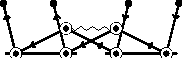
\includegraphics[height=0.84cm]{figs/ccd_d3a.pdf}
  };
\end{tikzpicture}
+
\begin{tikzpicture}[baseline=-2.5pt,every node/.style={inner sep=0pt,outer sep=0pt}]
  \node at (0,0) {
    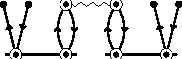
\includegraphics[height=0.84cm]{figs/ccd_d3b.pdf}
  };
\end{tikzpicture}
+
\begin{tikzpicture}[baseline=-2.5pt,every node/.style={inner sep=0pt,outer sep=0pt}]
  \node at (0,0) {
    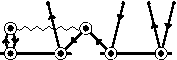
\includegraphics[height=0.84cm]{figs/ccd_d3d.pdf}
  };
\end{tikzpicture}
+
\begin{tikzpicture}[baseline=-2.5pt,every node/.style={inner sep=0pt,outer sep=0pt}]
  \node at (0,0) {
    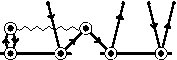
\includegraphics[height=0.84cm]{figs/ccd_d3c.pdf}
  };
\end{tikzpicture}
+
\begin{tikzpicture}[baseline=-2.5pt,every node/.style={inner sep=0pt,outer sep=0pt}]
  \node at (0,0) {
    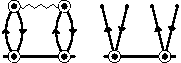
\includegraphics[height=0.84cm]{figs/ccd_d3e.pdf}
  };
\end{tikzpicture}
\\
\updownarrow\hspace{1pt}&
\\
  \tfr{1}{2}
  \ip{\F_{ij}^{ab}|H_\mr{c}\,T_2^2|\F}
=&\
  (\tfr{1}{2})^2\,
  \ol{g}_{kl}^{cd}
  t_{ab}^{kl}
  t_{cd}^{ij}
+
  \tfr{1}{2}
  \op{P}^{(a/b)}_{(i/j)}
  \ol{g}_{kl}^{cd}
  t_{ac}^{ik}
  t_{db}^{lj}
-
  \tfr{1}{2}
  \op{P}_{(a/b)}\,
  \ol{g}_{kl}^{cd}
  t_{ca}^{kl}
  t_{db}^{ij}
-
  \tfr{1}{2}
  \op{P}^{(i/j)}
  \ol{g}_{kl}^{cd}
  t_{cd}^{ki}
  t_{ab}^{lj}
+
  E_\mr{c}\,
  t_{ab}^{ij}
\end{align*}
In the last term, we have substituted in the CCD energy expression, which is the same graph as the CID energy expression.
\begin{align}
  E_\mr{c}
=
\diagram[top, bottom]{
%middle
  \node at (0,0.3) {
  $\left(
  \diagram{
    \draw (-0.5,0) node[circlex](f){} -- (0,0) node[ddot=white](f1){};
    \draw[->-] (f1) to ++(0,+0.5);
    \draw[-<-] (f1) to ++(0,-0.5);
  }
  +
  \diagram{
    \interaction{2}{g}{(0,0)}{ddot=white}{sawtooth};
    \draw[->-] (g1) to ++(0,+0.5);
    \draw[-<-] (g1) to ++(0,-0.5);
    \draw[->-] (g2) to ++(0,+0.5);
    \draw[-<-] (g2) to ++(0,-0.5);
  }\right)$
  };
%bottom
  \node at (0,-0.5) {
  $
  \mr{exp}
  \left(
  \diagram{
    \interaction{2}{c}{(0,-0.25)}{ddot}{overhang};
    \draw[->-] (c1) to ++(-0.25,+0.5);
    \draw[-<-] (c1) to ++(+0.25,+0.5);
    \draw[->-] (c2) to ++(-0.25,+0.5);
    \draw[-<-] (c2) to ++(+0.25,+0.5);
  }
  \right)$
  };
}
=
\diagram{
  \interaction{2}{g}{(0,+0.5)}{ddot}{sawtooth};
  \interaction{2}{c}{(0,-0.5)}{ddot}{overhang};
  \draw[-<-,bend right] (g1) to (c1);
  \draw[->-,bend left ] (g1) to (c1);
  \draw[-<-,bend right] (g2) to (c2);
  \draw[->-,bend left ] (g2) to (c2);
}
=
  (\tfr{1}{2})^2
  \ol{g}_{ij}^{ab}
  t_{ab}^{ij}
\end{align}
Note that the term $E_\mr{c} t_{ab}^{ij}$ actually cancels with the right-hand side of the projected Schr\"odinger equation.
Since this is the only unlinked graph in the expansion, we can write the amplitude equation as
\begin{align}
  \ip{\F_{ij}^{ab}|H_\mr{c}\mr{exp}(T_2)|\F}_\mr{L}
=
  0
\end{align}
where the subscript indicates that only linked graphs are included.
This cancellation of unlinked terms is a general feature of coupled-cluster theory.
Finally, note that when Brillouin's theorem holds the second and third terms in eq~\ref{eq:cid-coefficient-equations} become
\begin{align*}
  \op{P}_{(a/b)}
  f_a^c
  t_{cb}^{ij}
-
  \op{P}^{(i/j)}
  f_k^i
  f_{ab}^{kj}
=
-
  (\ev_i + \ev_j - \ev_a - \ev_b)
  t_{ab}^{ij}
\end{align*}
where $\{\ev_p=f_p^p\}$ are canonical Hartree-Fock orbital energies.
Subtracting this contribution from both sides leads to
\begin{align}
\label{eq:ccd-amplitude-equation-final}
  t_{ab}^{ij}
=
  (\mc{E}_{ab}^{ij})^{-1}
  \ip{\F_{ij}^{ab}|(H_\mr{c} - f_p^p\tl{a}^p_p)\mr{exp}(T_2)|\F}_\mr{L}
&&
  \mc{E}_{ab}^{ij}
\equiv
  \ev_i + \ev_j - \ev_a - \ev_b
\end{align}
which is the standard form for the $T_2$ amplitude equation.
\end{ex}

\begin{dfn}
\thmtitle{Resolvent line}
Complete contractions through a  \textit{resolvent line}
$
\resolventline[0.6]{}\hspace{3pt}
$
are defined as follows.
\begin{align*}
&&
  \gno{
  \ctr[4]
    {}
    {a}
    {^{i_1}\cd a^{i_k}a_{a_1}\cd a_{a_k}\,a^{b_1}\cd a^{b_k}a_{j_1}\cd }
    {a}
  \ctr[3]
    {a^{i_1}\cd}
    {a}
    {^{i_k}a_{a_1}\cd a_{a_k}\,a^{b_1}\cd a^{b_k}}
    {a}
  \ctr[2]
    {a^{i_1}\cd a^{i_k}}
    {a}
    {_{a_1}\cd a_{a_k}\,a^{b_1}\cd}
    {a}
  \ctr[1]
    {a^{i_1}\cd a^{i_k}a_{a_1}\cd}
    {a}
    {_{a_k}\,}
    {a}
  a^{i_1}\cd a^{i_k}
  a_{a_1}\cd a_{a_k}
  \resolventline[1.3]{}\,
  a^{b_1}\cd a^{b_k}
  a_{j_1}\cd a_{j_k}
  }
\equiv
  \fr{\gno{
    \ctr[4]
      {}
      {a}
      {^{i_1}\cd a^{i_k}a_{a_1}\cd a_{a_k}a^{b_1}\cd a^{b_k}a_{j_1}\cd }
      {a}
    \ctr[3]
      {a^{i_1}\cd}
      {a}
      {^{i_k}a_{a_1}\cd a_{a_k}a^{b_1}\cd a^{b_k}}
      {a}
    \ctr[2]
      {a^{i_1}\cd a^{i_k}}
      {a}
      {_{a_1}\cd a_{a_k}a^{b_1}\cd}
      {a}
    \ctr[1]
      {a^{i_1}\cd a^{i_k}a_{a_1}\cd}
      {a}
      {_{a_k}}
      {a}
    a^{i_1}\cd a^{i_k}
    a_{a_1}\cd a_{a_k}
    a^{b_1}\cd a^{b_k}
    a_{j_1}\cd a_{j_k}
  }}{
    \mc{E}_{a_1\cd a_k}^{i_1\cd i_k}
  }
&&
  \mc{E}_{a_1\cd a_k}^{i_1\cd i_k}
\equiv
  \sum_{r=1}^k
  \ev_{i_r}
-
  \sum_{r=1}^k
  \ev_{a_r}
\end{align*}
This can be denoted in a graph by drawing a horizontal dotted line through several contraction lines.
\end{dfn}

\newpage
\begin{ex}
Using the notion of a resolvent line, equation \ref{eq:ccd-amplitude-equation-final} can be written in diagram notation as follows.
\begin{align}
\nonumber
\diagram{
  \interaction{2}{t}{(0,-0.5)}{ddot}{overhang};
  \draw[->-] (t1) to ++(-0.25,1) node[dot] {};
  \draw[-<-] (t1) to ++(+0.25,1) node[dot] {};
  \draw[->-] (t2) to ++(-0.25,1) node[dot] {};
  \draw[-<-] (t2) to ++(+0.25,1) node[dot] {};
}
=&\
\diagram{
  \interaction{2}{g}{(0,-0.5)}{ddot}{sawtooth};
  \draw[->-] (g1) to ++(-0.25,1) node[dot] {};
  \draw[-<-] (g1) to ++(+0.25,1) node[dot] {};
  \draw[->-] (g2) to ++(-0.25,1) node[dot] {};
  \draw[-<-] (g2) to ++(+0.25,1) node[dot] {};
  \draw[thick,flexdotted] (-0.4,+0.35) to ++(1.8,0);
}
+
\diagram{
  \interaction{2}{t}{(0,-0.5)}{ddot}{overhang};
  \draw[->-=0.25,->-=0.75] (t1) to node[midway,ddot] (g1) {}
    ++(-0.25,1) node[dot] {};
  \draw[-<-=0.7] (t1) to ++(+0.25,1) node[dot] {};
  \draw[->-=0.25,->-=0.75] (t2) to node[midway,ddot] (g2) {}
    ++(-0.25,1) node[dot] {};
  \draw[-<-=0.7] (t2) to ++(+0.25,1) node[dot] {};
  \draw[sawtooth] (g1)--(g2);
  \draw[thick,flexdotted] (-0.4,+0.35) to ++(1.8,0);
}
+
\diagram{
  \interaction{2}{t}{(0,-0.5)}{ddot}{overhang};
  \draw[-<-=0.25,-<-=0.75] (t1) to node[midway,ddot] (g1) {}
    ++(-0.25,1) node[dot] {};
  \draw[->-=0.7] (t1) to ++(+0.25,1) node[dot] {};
  \draw[-<-=0.25,-<-=0.75] (t2) to node[midway,ddot] (g2) {}
    ++(-0.25,1) node[dot] {};
  \draw[->-=0.7] (t2) to ++(+0.25,1) node[dot,label] {};
  \draw[sawtooth] (g1)--(g2);
  \draw[thick,flexdotted] (-0.4,+0.35) to ++(1.8,0);
}
+
\diagram{
  \interaction{2}{t}{(0,-0.5)}{ddot}{overhang};
  \interaction{2}{g}{(1,+0.0)}{ddot}{sawtooth};
  \draw[->-] (t1) to ++(-0.25,1) node[dot,label] {};
  \draw[-<-] (t1) to ++(+0.25,1) node[dot,label] {};
  \draw[->-,bend left] (t2) to (g1);
  \draw[-<-,bend right] (t2) to (g1);
  \draw[->-] (g2) to ++(-0.25,0.5) node[dot] {};
  \draw[-<-] (g2) to ++(+0.25,0.5) node[dot] {};
  \draw[thick,flexdotted] (-0.4,+0.35) to ++(2.8,0);
}
+
\diagram{
  \interaction{2}{ta}{(0,-0.5)}{ddot}{overhang};
  \interaction{2}{tb}{(2,-0.5)}{ddot}{overhang};
  \interaction{2}{g}{(1,0)}{ddot}{sawtooth};
  \draw[->-=0.7] (ta1) to ++(-0.25,1) node[dot] {};
  \draw[-<-=0.3] (ta1) to (g1);
  \draw[->-=0.7] (ta2) to ++(-0.25,1) node[dot] {};
  \draw[-<-=0.3] (ta2) to (g2);
  \draw[->-=0.3] (tb1) to (g1);
  \draw[-<-=0.7] (tb1) to ++(+0.25,1) node[dot] {};
  \draw[->-=0.3] (tb2) to (g2);
  \draw[-<-=0.7] (tb2) to ++(+0.25,1) node[dot] {};
  \draw[thick,flexdotted] (-0.4,+0.35) to ++(3.8,0);
}
\\&\
\label{eq:ccd-amplitude-equations-final-diagrammatic}
+
\diagram{
  \interaction{2}{ta}{(0,-0.5)}{ddot}{overhang};
  \interaction{2}{tb}{(2,-0.5)}{ddot}{overhang};
  \interaction{2}{g}{(1,0)}{ddot}{sawtooth};
  \draw[->-] (ta1) to ++(-0.25,1) node[dot] {};
  \draw[-<-] (ta1) to ++(+0.25,1) node[dot] {};
  \draw[->-,bend left]  (ta2) to (g1);
  \draw[-<-,bend right] (ta2) to (g1);
  \draw[->-,bend left]  (tb1) to (g2);
  \draw[-<-,bend right] (tb1) to (g2);
  \draw[->-] (tb2) to ++(-0.25,1) node[dot] {};
  \draw[-<-] (tb2) to ++(+0.25,1) node[dot] {};
  \draw[thick,flexdotted] (-0.4,+0.35) to ++(3.8,0);
}
+
\diagram{
  \interaction{2}{ta}{(0,-0.5)}{ddot}{overhang};
  \interaction{2}{tb}{(2,-0.5)}{ddot}{overhang};
  \draw[sawtooth] (0,0) node[ddot] (g1) {} to (1.5,0) node[ddot] (g2) {};
  \draw[->-,bend left]  (ta1) to (g1);
  \draw[-<-,bend right] (ta1) to (g1);
  \draw[->-=0.7] (ta2) to ++(-0.25,1) node[dot] {};
  \draw[-<-] (ta2) to (g2);
  \draw[->-] (tb1) to (g2);
  \draw[-<-=0.7] (tb1) to ++(+0.25,1) node[dot] {};
  \draw[->-] (tb2) to ++(-0.25,1) node[dot] {};
  \draw[-<-] (tb2) to ++(+0.25,1) node[dot] {};
  \draw[thick,flexdotted] (0.6,+0.35) to ++(2.8,0);
}
+
\diagram{
  \interaction{2}{ta}{(0,-0.5)}{ddot}{overhang};
  \interaction{2}{tb}{(2,-0.5)}{ddot}{overhang};
  \draw[sawtooth] (0,0) node[ddot] (g1) {} to (1.5,0) node[ddot] (g2) {};
  \draw[->-,bend left]  (ta1) to (g1);
  \draw[-<-,bend right] (ta1) to (g1);
  \draw[-<-=0.7] (ta2) to ++(-0.25,1) node[dot] {};
  \draw[->-] (ta2) to (g2);
  \draw[-<-] (tb1) to (g2);
  \draw[->-=0.7] (tb1) to ++(+0.25,1) node[dot] {};
  \draw[-<-] (tb2) to ++(-0.25,1) node[dot] {};
  \draw[->-] (tb2) to ++(+0.25,1) node[dot] {};
  \draw[thick,flexdotted] (0.6,+0.35) to ++(2.8,0);
}
\end{align}
\end{ex}

\begin{rmk}
\thmtitle{The CEPA$_0$ and MP2 amplitude equations}
If the $T_2$ amplitudes are small
\begin{align}
  \text{MP2}:\hspace{5pt}
  t_{ab}^{ij}
\approx
  (\mc{E}_{ab}^{ij})^{-1}
  \ip{\F|V|}
\end{align}
\end{rmk}


\end{document}